\chapter{Project Design}
The tools that are used in this paper are mostly Python-based, such as TensorFlow, a neural network framework. This, combined with natural language processing tools and several filtering techniques will be used to achieve -- or at least approach as close as possible to -- the expected results.
Having all the concepts in mind, the proposed project has a major component which is the Machine Learning tools surrounded by several small modules such as the GUI and the chatbot components.
As for the data used in this project, most of it comes from cleaned, classified tweets partitioned in training and testing datasets.
In this chapter, the design of the project is explained.

\section{Inner Workings Design}
In this section, the data and the relations with the algorithm is explained, with a focus on the design itself.
\subsection{Datasets}
The datasets used in this project, as previously mentioned, consist in around 40,000 semi-clean, classified tweets in 13 categories \citep{rf20}, but as the scope for all of those labels exceeds the one proposed in this paper, the ones taken into consideration are as follows:
\begin{itemize}
	\item Sadness
	\item Neutral
	\item Happiness
	\item Fun
	\item Worry
	\item Boredom
\end{itemize}
Even after eliminating non-critical labels, since the remaining  labeled samples are not evenly distributed, leaving them as-is led to very inaccurate results, so a generalistic approach was opted for, classifying the end results in ``Good'', ``Neutral'' and ``Bad'' depending on the overall wellness percieved from the input.
This final filter works only with the training data, and works as follows:
\begin{itemize}
	\item Sadness and Worry are in the ``Bad'' category.
	\item Neutral and Boredom are in the ``Neutral'' category.
	\item Happiness and Fun are in the ``Good'' category.
\end{itemize}

\subsection{Text Filtering}
Since the chosen dataset is imported almost straight from Twitter with poor grammar, misplaced symbols, emojis and similar things, some cleanup has to be done to ensure peak performance.
\begin{itemize}
\item First, all text must be converted to lowercase.
\item Then, all of the punctuation marks had to be discarded.
\item After that, the stopwords\footnote{Words that are not vital for the sentence's meaning.} have to be omitted as well.
\item Finally, for easier analysis, a process called stemming\footnote{Reducing a verb to its most basic components.} is applied, so that all of the tenses of every verb are evaluated the same way while also avoiding corpus bloating.
\end{itemize} 
These last processes were possible thanks to NLTK\footnote{Natural Language Toolkit, tool used specifically for these case scenarios. \url{https://www.nltk.org/}}, which has its own repository of stopwords and stems.
An example for this applied to data in the training dataset is as follows.
\begin{center}
\fbox{So sleepy again and it's not even that late. I fail once again.}
\end{center}
Following the filtering order, first all the characters are converted to lowercase.
\begin{center}
\fbox{so sleepy again and it's not even that late. i fail once again.}
\end{center}
After that, the text is stripped from all non-alphabetic characters.
\begin{center}
\fbox{so sleepy again and it s not even that late i fail once again}
\end{center}
Next, all stopwords are culled from the sentence.
\begin{center}
\fbox{sleepy even late fail}
\end{center}
The last step is to apply stemming to all the able remaining words, in this case, the adjective ``sleepy'' stems from sleep.
\begin{center}
\fbox{sleepi even late fail}
\end{center}


\subsection{Neural Network}
For this project, as mentioned in Chapter 3, TensorFlow was opted for because of its characteristics such as being free to use, not needing a lot of resources to work and the advantages of being portable once trained. All of these traits are what makes this project unique and easily scalable.
An LSTM Neural Network was opted for because of the increased accuracy that it offers compared to a regular Recurrent Neural Network.
\begin{figure}[!b]
	\centering
	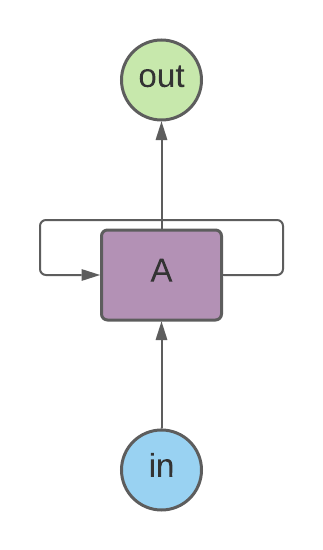
\includegraphics[scale=0.7]{Normal_RNN}
	\caption{Basic Structure of a Recurrent Neural Network, where \textit{A} represents the algorithm used.}
	\label{fig:neuraldiagram_1}
\end{figure}
\begin{figure}[!bht]
	\centering
	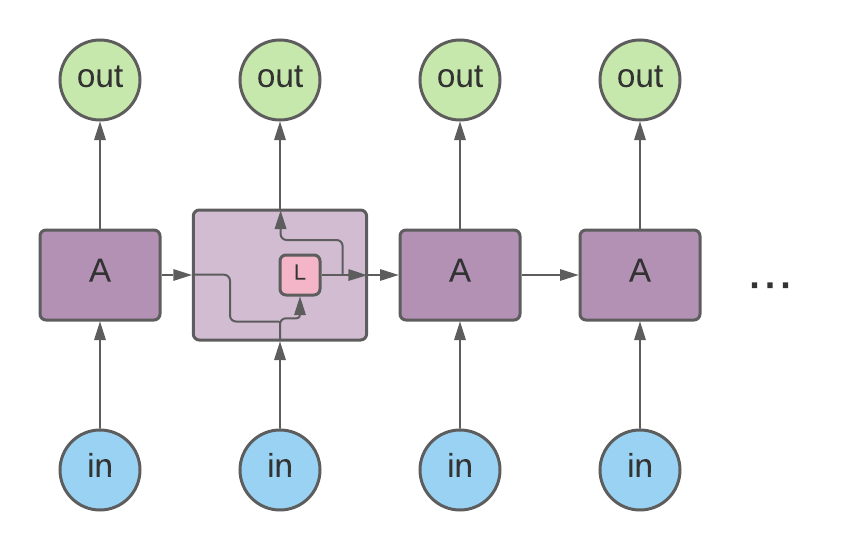
\includegraphics[scale=0.7]{Transp_RNN}
	\caption{Structure inside an algorithm in a basic Recurrent Neural Network, where \textit{L} represents the layers used.}
	\label{fig:neuraldiagram_2}
\end{figure}
\\
\indent Basically, LSTM is a subtype of a Recurrent Neural Network which has a certain amount of data be stored for longer periods of time so it can be used for future connections.
\begin{figure}[!bht]
	\centering
	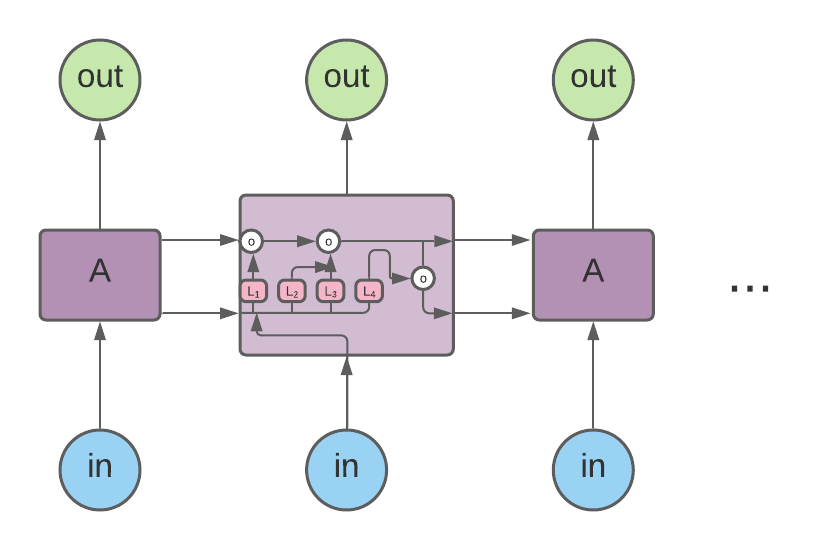
\includegraphics[scale=0.7]{Transp_LSTM}
	\caption{Structure inside an LSTM Neural Network, where the \textit{o} represent the functions that operate the data the data when traveling from one layer to another \citep{rf21}.}
	\label{fig:neuraldiagram_3}
\end{figure}
\pagebreak
\section{Tools}
This project is built on Python v3.8.10, The libraries used for this project to come to fruition are TensorFlow\footnote{\url{https://www.tensorflow.org/}} v2.6.0 and Keras\footnote{\url{https://keras.io/}} v2.6.0 for the Neural Network section. Natural Language Toolkit\footnote{\url{https://www.nltk.org/}} v3.5 (also known as NLTK) for the tokenization and stemming process. Chatterbot\footnote{\url{https://chatterbot.readthedocs.io/en/stable/}} for the chatbot's output. And, lastly, pygame\footnote{\url{https://www.pygame.org/news}} v1.9.5 for the GUI.
Originally, \textit{Ren'py}\footnote{An open-source Python framework focused mostly in the development of visual novels and other videogame formats. \url{https://www.renpy.org/}} was the chosen framework for this project's interface to work with, but -- unfortunately for the proposed usage -- it only works with Python 2.7, which makes it incompatible with TensorFlow 2.0. Making a bridge between Python 2 and 3 would inevitably generate more issues that would take more time to solve, so it was scrapped in favor of the pygame library.

\section{Interface}
Originally, \textit{Ren'py}\footnote{An open-source Python framework focused mostly in the development of visual novels and other videogame formats. \url{https://www.renpy.org/}} was the chosen framework for this project's interface to work with, but -- unfortunately for the proposed usage -- it only works with Python 2.7, which makes it incompatible with TensorFlow 2.0. Making a bridge between Python 2 and 3 would inevitably generate more issues that would take more time to solve, so it was scrapped in favor of the \textit{pygame} library.
\pagebreak

\begin{figure}[!h]
	\centering
	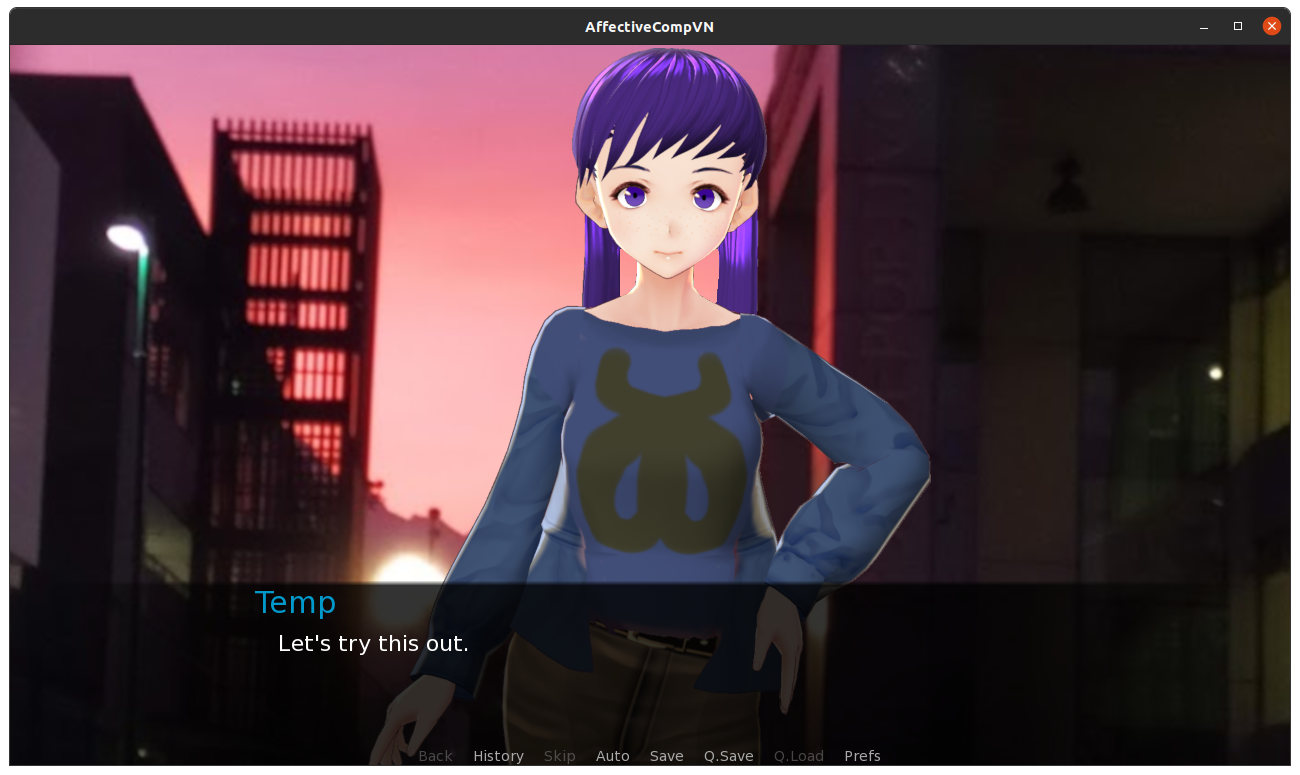
\includegraphics[scale=0.3]{Ren'py}
	\caption{First version of the interface using Ren'py.}
	\label{fig:renpy_test_1}
\end{figure}
\begin{figure}[!h]
	\centering
	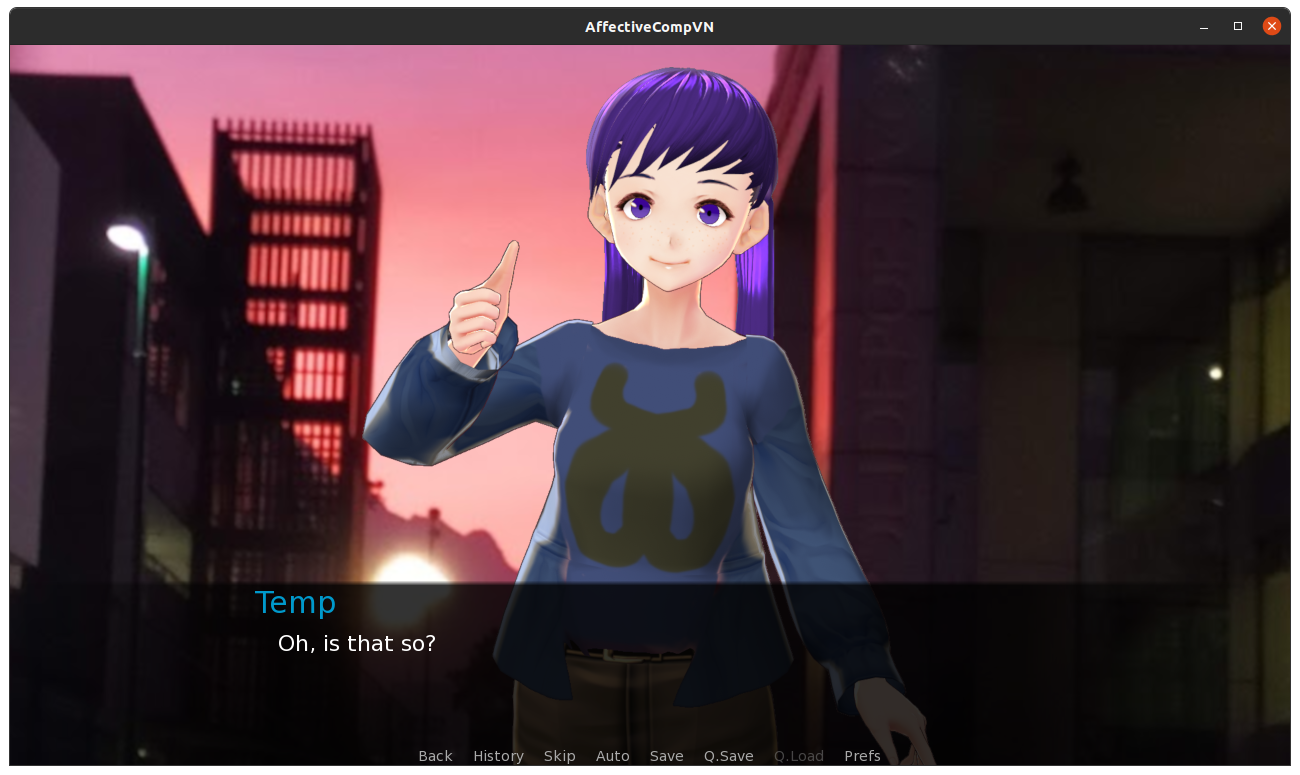
\includegraphics[scale=0.3]{Ren'py_2}
	\caption{Reacting positively to text in the ``Good'' category in the Ren'py version.}
	\label{fig:renpy_test_2}
\end{figure}

The current interface is a hybrid between a Pygame screen, where the assistant appears to react to the input, and the console, where a person can input text to be analyzed.

\begin{figure}[!h]
	\centering
	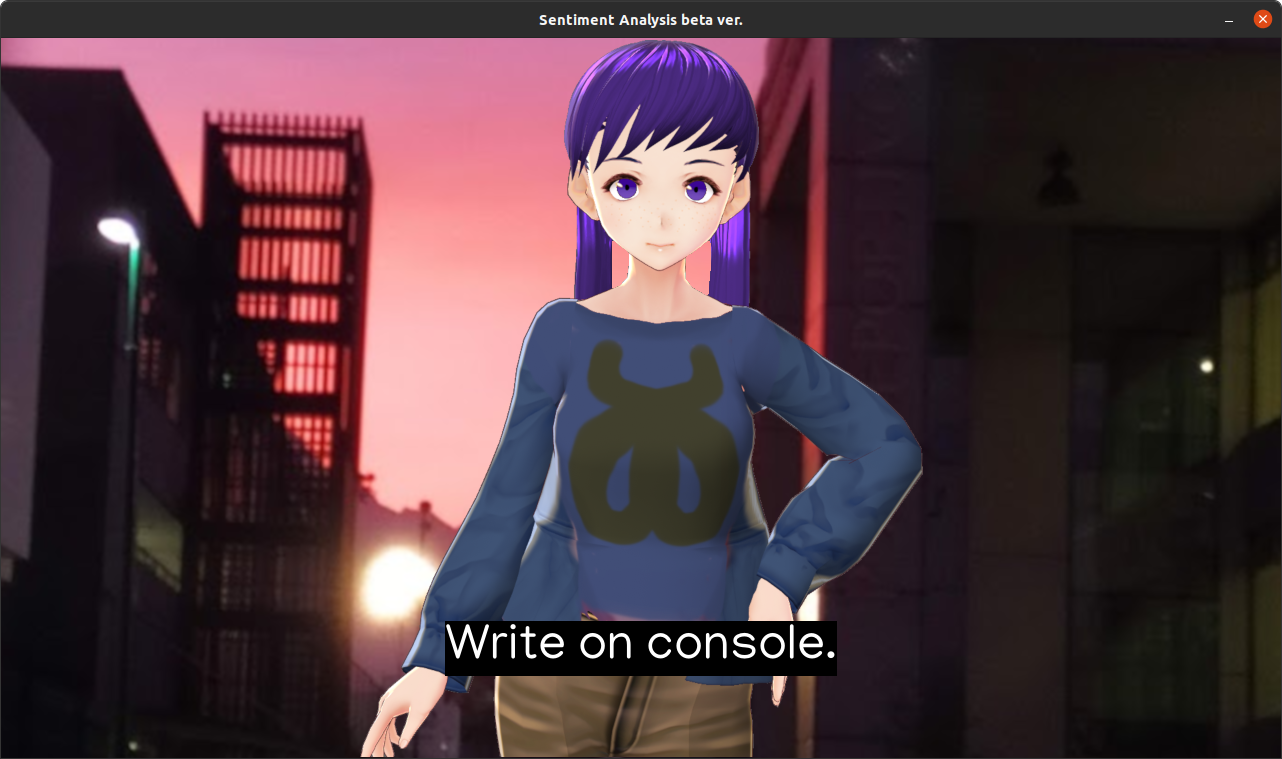
\includegraphics[scale=0.3]{PyGame1}
	\caption{Current version of the interface, using PyGame}
	\label{fig:PyGame1}
\end{figure}
\begin{figure}[!h]
	\centering
	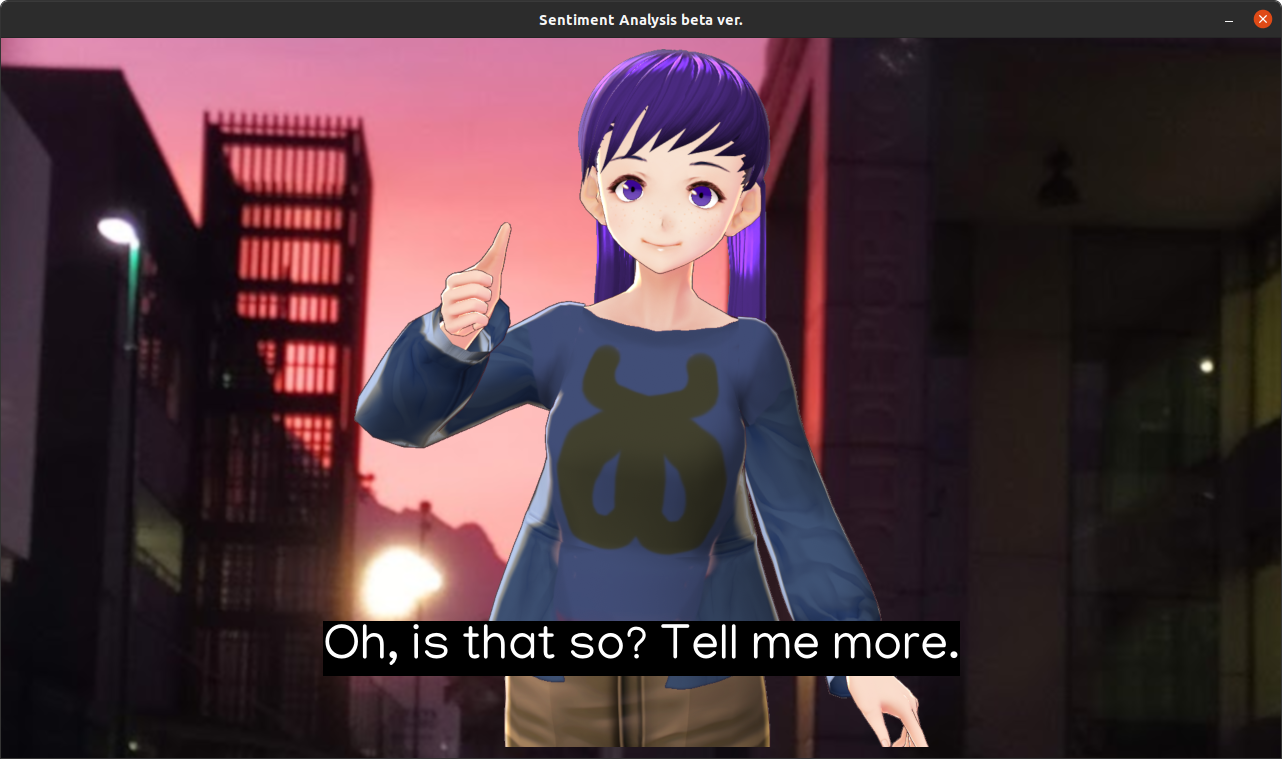
\includegraphics[scale=0.3]{PyGame2}
	\caption{Reacting positively to text in the ``Good'' category in the PyGame version.}
	\label{fig:PyGame2}
\end{figure}

\subsection{Assistant}
As for the character that is being used, it also has gone through some changes. Originally the idea was to make a low-poly character render to work with, but since 3D modeling-from-scratch skills exceed the scope of this paper, an alternative software was selected instead. Namely \textit{VRoid}.\\
The main purpose for this assistant is to make people feel like it is her that they are talking to and not to some faceless machine, while also making it easier to the eyes. A more realistic, less animated style could have been used, but a friendly, less prone to uncanny valley approach to the design was opted for with this in mind.
\begin{figure}[!bht]
	\centering
	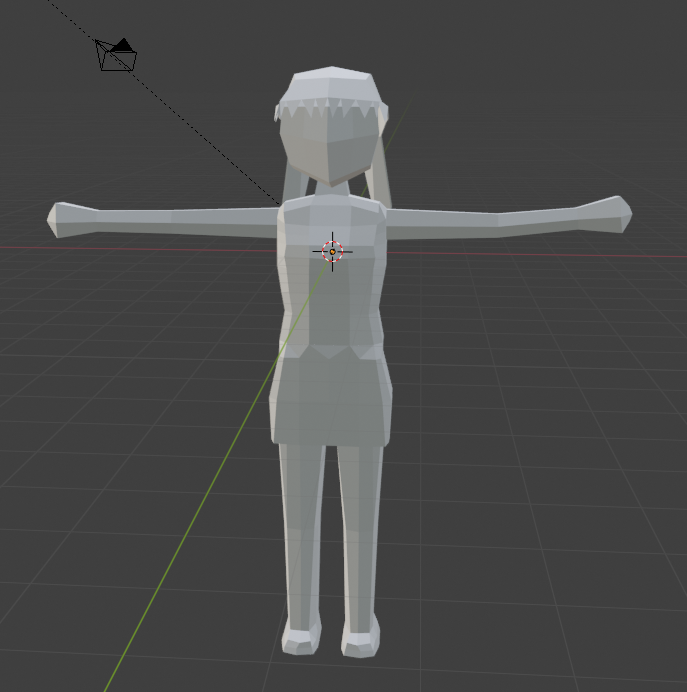
\includegraphics[scale=.5]{Assistant_1}
	\caption{First attempt at 3D modeling an assistant.}
	\label{fig:assistant1}
\end{figure}
\begin{figure}[!bht]
	\centering
	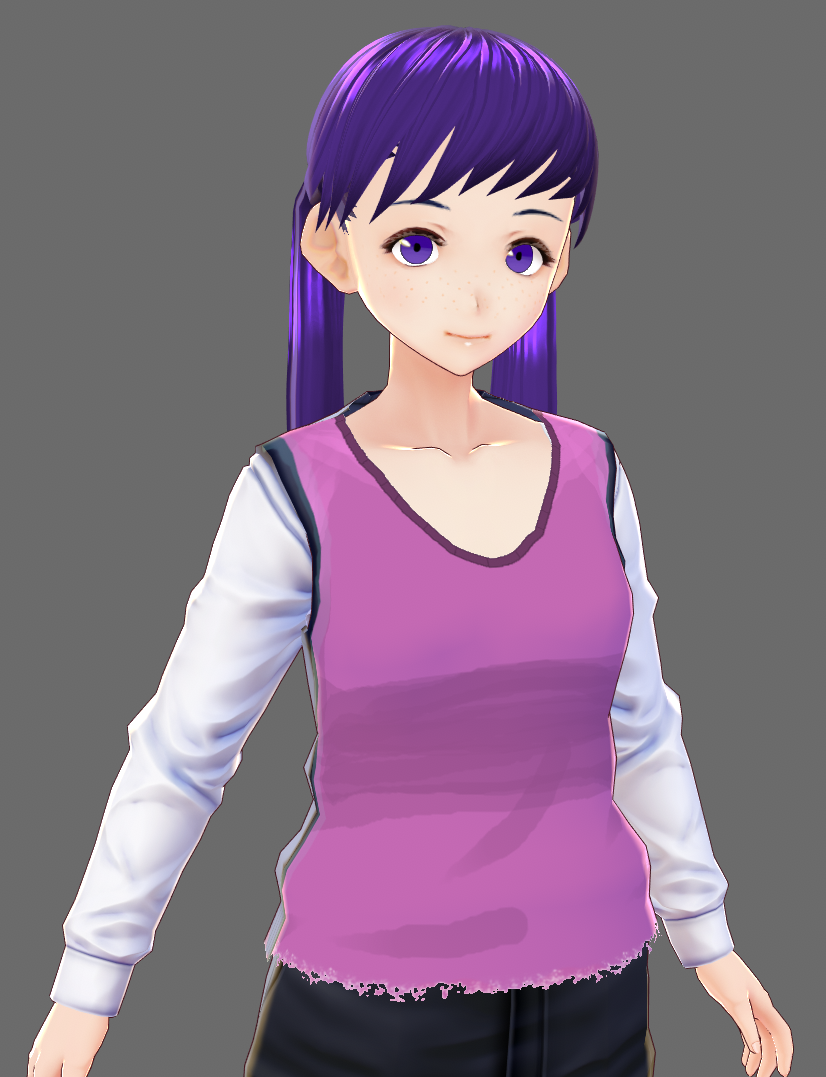
\includegraphics[scale=.25]{Assistant_2}
	\caption{Assistant Ver. 2, now using VRoid.}
	\label{fig:assistant2}
\end{figure}
\begin{figure}[!bht]
	\centering
	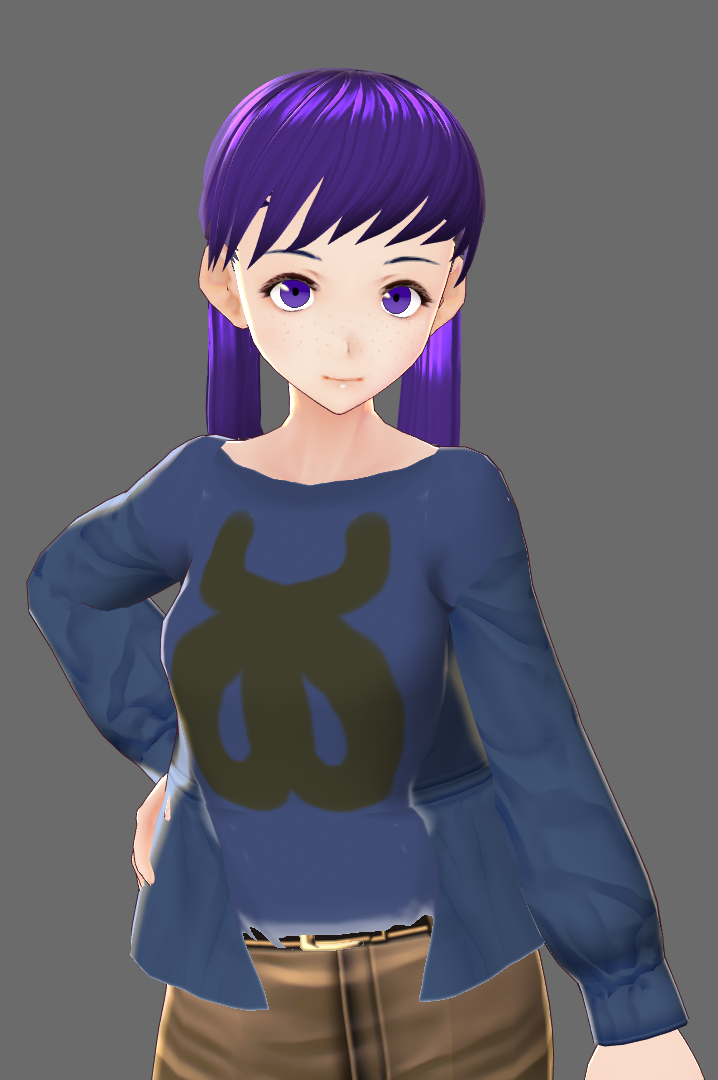
\includegraphics[scale=.25]{Assistant_3}
	\caption{Assistant Ver. 3, the current design.}
	\label{fig:assistant3}
\end{figure}
\pagebreak

\section{Inner Workings}
In this section, I will highlight the most important parts of this project's code and their function. In case of needing further insight on the code used, the repository is online at \url{https://github.com/Alex-Ego/Affective-Computing-VN}.
\subsection{Text Filtering}
After the dataset has been properly located and ready to be used, the cleanup discussed earlier in this chapter happens in the following code snippet:
\begin{lstlisting}
def tokenizing_process(message):
    # Pre-tokenizing
    tokens = word_tokenize(message)
    
    # Making them lowercase
    tokens = [w.lower() for w in tokens]
    
    # Filtering the punctuations
    table = str.maketrans('', '', string.punctuation)
    stripped = [w.translate(table) for w in tokens]
    
    # Filtering non-alphabetic characters
    words = [word for word in stripped if word.isalpha()]
    
    # Removing stopwords
    stop_words = set(stopwords.words('english'))
    words = [w for w in words if not w in stop_words]
    
    # Stemming words
    porter = PorterStemmer()
    stemmed = [porter.stem(word) for word in words]
    
    # Joining the resulting string
    message = " ".join(stemmed)
    return message
    
\end{lstlisting}
This works in the same way and order as specified earlier in this chapter.
\subsection{Neural Network}
After the text has been properly classified and ready-to-test, this is the structure of the neural network.
\begin{lstlisting}
model = tf.keras.Sequential([
    layers.Embedding(input_dim=vocab_size, 
                           output_dim=embedding_dim, 
                           input_length=max_length),
    layers.SpatialDropout1D(0.15),
    layers.Bidirectional(layers.LSTM(32, dropout=0.15,
recurrent_dropout=0.15)),
    layers.Dense(8, activation="tanh"),
    layers.Dense(4, activation="softmax")
])
\end{lstlisting}
As the code shown indicates, this neural network has 3 layers: LSTM for classification, and two Dense, the former is to slim down the input data from the previous layer, and the latter is for classification which can be one in 4 categories, which include the three previously discussed categories, and one reserved for error/unknown purposes.
\subsection{Portability}
Training the Neural Network every time is not needed, since there is a way to save the model in a \textit{.hdf5} file and the corpus in a plain \textit{.txt} file with the following code snippet:
\begin{lstlisting}
model_location = os.path.join(abs_location, "nndata/model")
keras.models.save_model(model, model_location + 
"/sentimental_analysis.hdf5")
with open(model_location + "/tokens.txt", "w") as f:
    f.write(tokenizer.to_json())
    f.close()
\end{lstlisting}
This is fairly useful, because training it every time is very time and resource consuming. Having this as an option opens the path for more applications in less powerful systems.